\subsubsection{Part A}
Using the circuit shown in figure (\ref{fig:pmos_circuit}), $I_{sd}$ is measured as the drain voltage is varied from within the range of $0 V \le V_{sd} \le 5 V$. 
The value of the gate voltage is set to $V_{sg} = 2.5V$. 
\\

\FloatBarrier

\begin{figure}[h!]
	\centering
	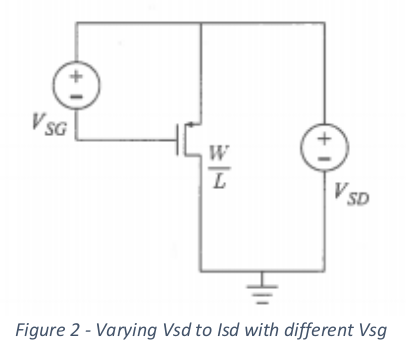
\includegraphics[scale=0.75]{./images/pmos_circuit}
	\caption{The PMOS transistor circuit used for our measurements.}
	\label{fig:pmos_circuit}
\end{figure}

\FloatBarrier
From the $I_{sd}$ vs $V_{sd}$ curve in figure (\ref{fig:pmos}), this PMOS transistor is not active until $V_{sd} \approx 1.8 V$. This region should not be called cutoff mode since cutoff mode implies that $V_{sg}$ is too low. The transistor simply does not operate below the determined $V_{sd}$, which is not consistent with theory.

\FloatBarrier

\begin{figure}[h!]
	\centering
	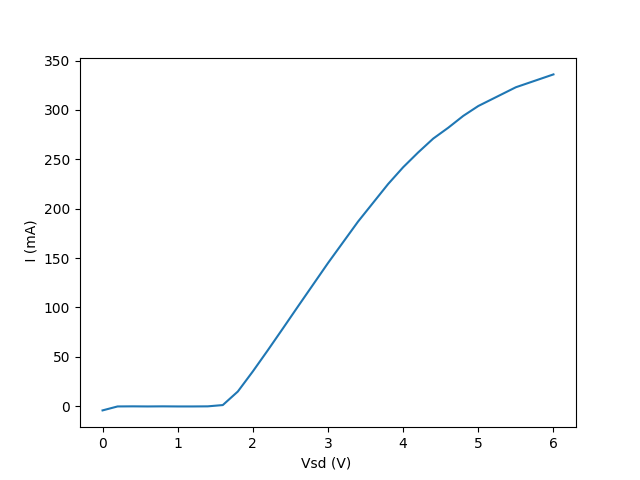
\includegraphics[scale=0.75]{./data/pmos.png}
	\caption{The resulting $I_{sd}$ vs $V_{sd}$ graph for $V_{sg}=2.5V$}
	\label{fig:pmos}
\end{figure}

\FloatBarrier
To turn on this transistor the gate voltage must be greater than the source voltage by at least the absolute value of the threshold voltage. 
This means that at $V_{sd} = 1.8 V$, $V_{sg} \ge |V_{tp}|$.
\\

To operate in triode mode $V_{sd}$ must be less than $V_{sg}$ by at least the absolute value of the threshold voltage.
The transistor operates in the triode mode for $ V_{sd} \ge 1.8V$.
Given that the data does not show signs of entering saturation mode, it is not possible to find the saturation edge from the data alone.
\\

\subsubsection{Part B}
Part B uses the same procedure as part A, but the gate voltage is changed to $V_{sg} = 5 V$. 

\FloatBarrier

\begin{figure}[h!]
	\centering
	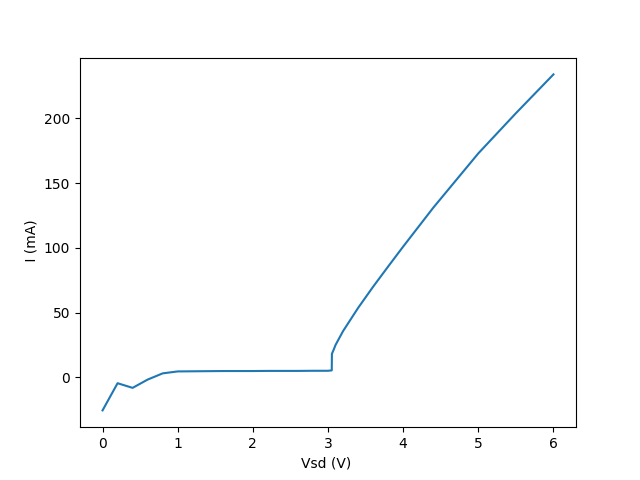
\includegraphics[scale=0.75]{./data/pmos_5v.png}
	\caption{The resulting $I_{sd}$ vs $V_{sd}$ graph for $V_{sg}=5V$}
	\label{fig:pmos_5v}
\end{figure}

\FloatBarrier
Much like in part A, the transistor is strangely inactive until $V_{sd} = 3.05 V$. This behavior cannot be explained using this lab's currently accepted transistor models and theory.
It then operates in triode mode for the rest of the values tested up to $V_{sd}=6V$.
Given that the data does not show signs of entering saturation mode, the saturation edge cannot be determined without further analysis.
